\documentclass[11pt,a4paper]{article}
\usepackage[margin=2cm]{geometry}
\usepackage[affil-it]{authblk}

\usepackage{graphicx}
\usepackage{booktabs} % for fancier table lines

\usepackage{float} %to fix figure positions

\usepackage[T1]{fontenc}
\usepackage[utf8]{inputenc}
\usepackage[hidelinks]{hyperref} % for hyperlinks (both in and out the paper)
\usepackage{amsmath}
\usepackage{paralist}
\usepackage{natbib}
\usepackage{color}
\usepackage[mathlines]{lineno} % for line numbers
\linespread{1}
\usepackage{wrapfig}

\usepackage{multirow}

\usepackage[labelfont=bf,font=footnotesize]{caption} % for the figure and table captions
\setlength{\abovecaptionskip}{2pt} 
\setlength{\belowcaptionskip}{-5pt}

\usepackage{indentfirst} % to indent first paragrpah of each sentence
\setlength\parindent{0.3cm}

%%%%%%%%% Keep this block in manuscript to allow commenting %%%%%%%%%
\usepackage{color}
\usepackage{setspace}
\usepackage{soul} %to get highlights with todo notes
\usepackage[backgroundcolor=yellow,textsize=tiny,textwidth=.7in]{todonotes}
% {\begin{spacing}{0.5}#2\end{spacing}}
\newcounter{todocounter}
\newcommand{\todonum}[2][]
{\stepcounter{todocounter}\todo[#1]{\thetodocounter: #2}}
\newcommand{\hlfix}[2]{\texthl{#1}\todonum{#2}~} %this needs the soul package
%%%%%%%%%%%%%%%%%%%%%%%%%%%%%%%%%%%%%%%%%%%%%%%%%%%%%%%%%%%%%%%%%%%%%%

%%%%%%%%%%%%%%%%%%%%%%%%%%%%%%%%%%%%%%%%%%%%%%%%%%%%%%%%%%%%%%%%%%%%%

\linenumbers

%%%%%%%%%%%%%%%%%%%%%%%%%%%%%%%%%%%%%%%%%%%%%%%%%%%%%%%%%%%% 

\title{Sensitivity of the thermal niche of arthropods to physiological mismatches between life stages}

\author{Samraat Pawar$^1$, Thomas R. C. Smallwood$^2$, Alex Chan$^1$, Marta Shocket$^3$, Lauren Cator$^1$}

\affil{$^1$Department of Life Sciences, Imperial College London, Silwood Park Campus, Ascot, UK 
$^2$Department of Infectious Disease Epidemiology, School of Public Health, Imperial College London, St Mary’s Campus, London, UK
$^3$\hl{Marta's affiliation}
}

\date{Version dated: \today}

%%%%%%%%%%%%%%%%%%%%%%%%%%%%%%%%%%%%%%%%%%%%%%%%%%%%%%%%%%%%

\begin{document}

\maketitle

%%%%%%%%%%%%%%
%% ABSTRACT %%
%%%%%%%%%%%%%%

\section*{Abstract}

Currently, there are widespread concerns about climate-driven changes in the population dynamics of economically-important arthropods such as disease vectors, pests, and pollinators. Arthropod population dynamics are strongly driven by environmental temperature and there is growing interest in understanding and predicting the effect of climatic variation on their abundances. However, most arthropods have stage-structured life histories, with the different life stages often experiencing different thermal environments, or differing inherently in their thermal physiology. Yet, we lack a quantitative framework for predicting how life stage-specific differences impact temperature-driven arthropod population dynamics. In this study, we combine life-history and ecological metabolic theory to model the intrinsic growth rate of arthropod populations under different levels of ``mismatch'' between the thermal responses of adult and juvenile life history traits. We show that mismatches between juvenile and adult life stages result in predictable shifts in the thermal optimum as well as niche width of fitness of the population. Specifically, we find that a 1$^\circ$C increase in temperature can increase the thermal optimum by xx, and thermal niche breadth between xx-xx percent. Furthermore, we empirically ground these theoretical results by performing a data-synthesis to show that thermal mismatches are likely to be common across the major arthropod taxa. Our study highlights the importance of physiological mismatches between different life stages in disease vector populations, need for empirical data, and further theoretical work on how life stage-specific thermal mismatches may amplify the effects of climate change on insect populations.

%%%%%%%%%%%%%%%%%%
%% INTRODUCTION %%
%%%%%%%%%%%%%%%%%%

\section*{Introduction}
Arthropods constitute approximately three-quarters of all known biological organisms (living or extinct) and inhabit virtually every known ecosystem. This group of animals is enormously important to the ecological health of the planet. For humans, this group is economically beneficial.Insects alone are estimated to provide more than  "Dollar sign" 57 billion in ecosystems services to the US economy (Cite Losey and Vaughan Bioscience 56, 311-323 (2006). At the same time, arthropods also represent one of the largest threats to human health and livelihood. Vector-borne diseases (VBDs), which are almost exclusively transmitted by arthropods, constitute approximately 17\% of infectious human disease incidence worldwide \citep{WHO2004}. In addition to directly impacting human health, many vector-borne plant diseases threaten food security \citep{Nault1997, Childers2003, Kitajima2003, Rodrigues2003}. 

Arthropod populations are currently experiencing dramatic changes in abundance. A recent study, reported that the current rates of decline will lead to the extinction of 40 "percent symbol" of the world's insect species over the next few decades. Climate was identified as an important driver of these declines. In order to understand how ecological factors such as temperature will alter abundances we need a better understanding of how temperature alters population growth dynamics. 

Arthropod metabolic traits are directly dependent on changes in environmental temperature \citep{Tabachnick2010,Amarasekare2012a}. Therefore, temperature variation strongly affects their population growth rate and abundance \citep{Amarasekare2012a,Angilletta2009}. The stage-structured life-cycles of arthropods make it particularly challenging to understand the temperature dependence of their population dynamics. One of the main reasons for this complexity is that temperature often affects life history traits of different life stages (e.g., fecundity, mortality and development rate) in different ways \citep{Amarasekare2013,Mordecai2012,Dell2011a,Parham2010,Lunde2013}. 

Such stage-specific differences are expected to be common because traits may not only differ inherently in their underlying thermal physiology (e.g., juvenile development vs. adult mortality rate), but also because different life-stages experience different thermal regimes. For example, the juvenile stages of mosquitoes develop in water, which may be as much as 6 $^\circ$C warmer than the environment experienced by adults \citep{Paaijmans2010d}, while the juvenile stages of tsetse flies ({\it Glossina} spp.) partly develop in the adult female and partly in the soil, which may be significantly warmer than air temperature \citep{Kleynhans2014}. Immature stages of vectors will typically be more affected as their lower motility results in a more limited ability to escape stressful temperatures than adults. The effects of differences in adult and juvenile thermal responses (Thermal Performance Curves, TPCs) of traits (or ``physiological mismatches'') remain largely unexplored theoretically and empirically (But see Dobson and Beck-Johnson, other citations?).

Here, we combine life-history and metabolic theory to model the intrinsic growth rate of arthropod populations under physiological mismatches --- a key parameter that quantifies exponential growth rate in population abundance \citep{Birch1948, Savage2004d, Amarasekare2012a}. Using this model, we assess the effect of mismatches on the thermal optimum and niche width of the thermal performance curve (TPC) of population growth rate (Fig \ref{fig:TPCModel}). We also use the model to quantify the relative contribution of juvenile vs. adult stages to population growth rate. While previous studies have focused on the thermal optimum, thermal niche width is also key for understanding arthropod  population dynamics in natural environments, where temperatures fluctuate over space and time \citep{Paaijmans2010d,Paaijmans2013} (add more citations here from non-vector examples).


%%%%%%%%%%%%%
%% METHODS %%
%%%%%%%%%%%%%

\section*{Methods} 

\subsection*{The population growth rate model}

Our growth model is based on the assumption that the population has a stable age distribution (SAD, i.e., the proportion of individuals in adult and juvenile life stages is constant). Under the SAD assumption the Euler-Lotka equation gives the expected reproductive success of a newborn individual in a population that growing at a rate $r_\text{m}$ \citep{Charnov1993a, Savage2004d, Amarasekare2012a, Amarasekare2013}:

\begin{equation}  \label{eq:EuLot}
	\int_\alpha^\infty  {{e^{ - {r_\text{m}}x}}{l_x}{b_x}dx}  = 1	
\end{equation}

Here, $\alpha$ is the age at first reproduction (development time; days needed for development from egg to adult), $l_x$ is age-specific survivorship (proportion of individuals that survive from birth to age $x$), and $b_x$ the age-specific fecundity (number of offspring produced by an individual of age $x$). 

Using the simplest feasible mortality and fecundity models (for $l_x$ and $b_x$ respectively) for insects, we then show that (Supplementary Information 1):
\begin{equation} \label{eq:rm_app}
	r_m \approx \frac{(\kappa + z)  \left( \log\left(\frac{b_\text{opt}}{\kappa + z} \right) - \alpha z_J\right)}{\alpha (\kappa + z) + 1}
\end{equation}
where $x_\text{opt}$ is the age of peak fecundity $b_\text{opt}$, $\kappa$ is age-specific fecundity loss rate (controls spread of the fecundity  schedule), $z_J$ is mortality rate averaged across all juvenile stages, and $z$ is adult mortality rate (SI1). Substituting models of the TPCs of these life history traits (see below) then gives the temperature dependence of $r_\text{m}$ (Table \ref{tab:traits}).


\subsection*{Temperature-dependence of life history traits}

Next we substitute the thermal responses of the component traits of $r_\text{m}$ (\ref{tab:traits}). We model each trait's temperature dependence using a modified Sharpe-Schoolfield equation \citep{Schoolfield1981}: 
   
\begin{equation} \label{eq:TPCModel}
B = B_0 \dfrac
{	e^{\dfrac{-E_\text{}}{k} \left (\dfrac{1}{T} - 
\dfrac{1}{T_\text{ref}} \right ) } }
{1 + \dfrac{E}{E_\text{D} - E}  e^{\dfrac{E_\text{D}}{k}  
\left (\dfrac{1}{T_\text{opt}} - \dfrac{1}{T} \right )}}
\end{equation}
Here, $B$ is the value of the metabolic trait at a given temperature $T$ (K), $B_{0}$ is a normalisation constant representing the value of the trait at some reference temperature $T_\text{ref}$, $E$ is the ``activation  energy'' (eV) which controls the rise of the curve up to the peak (initial thermal sensitivity), $T_\text{opt}$ is the temperature at which the trait value or rate is maximised, and $E_\text{D}$ is the de-activation energy (eV), which determines the rate at which the trait declines after the peak. The parameter $k$ is the universal Boltzmann constant ($8.617 \cdot 10^{-5}$ eV  $K^{-1}$). The constant $B_0$ also includes the effect of body size, and therefore the effect of stage-specific size differences.       

\begin{figure}[H] 
	\centering
	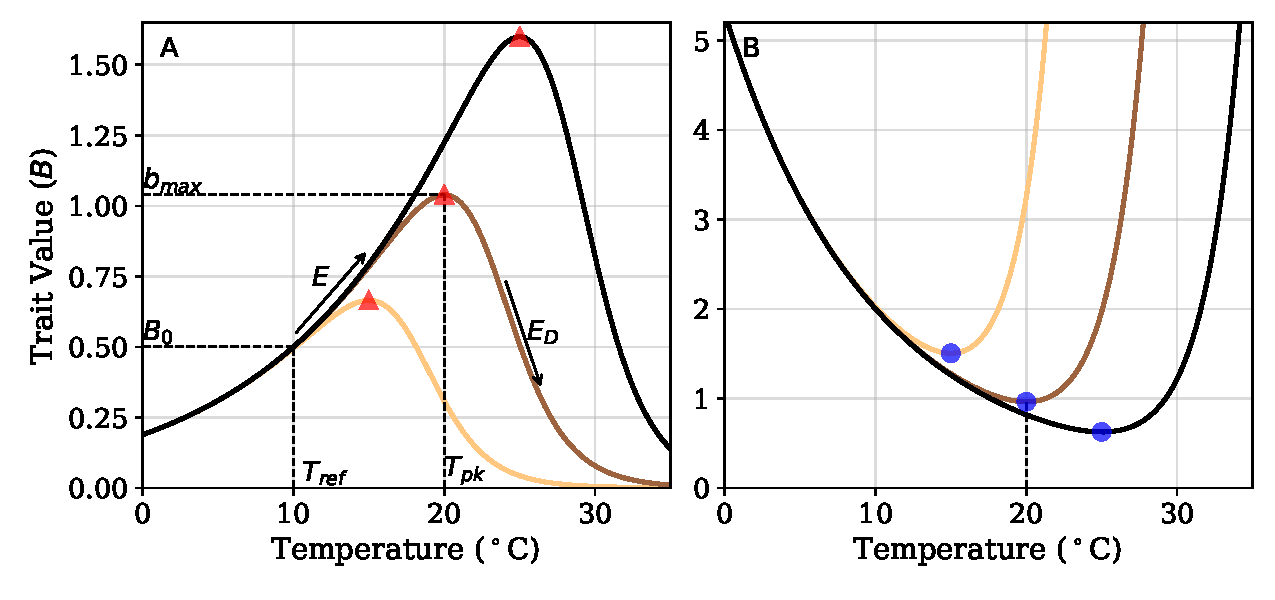
\includegraphics[width = .8\textwidth]{results/TPCModel.pdf}
	\caption{{\bf Illustration of the thermal performance curve (TPC) of vector life-history traits. A:} A Sharpe-Schoolfield model was used to generate TPCs for traits that are rates (peak fecundity rate, $b_\text{opt}$ and fecundity loss rate $\kappa$). {\bf B:} The inverse of this model (inverse of the curve in A) was used to generate TPCs for times (e.g., development time, $a$) or  non-unimodal rates (e.g., mortality rates $z$ and $z_J$). See Table \ref{tab:traits} for the list of traits. The vertical dotted line  marks $T_\text{opt}$ (the thermal optimum).}
\label{fig:TPCModel}
\end{figure} 

Equation \eqref{eq:TPCModel} has been used as a model for thermal performance of traits in numerous previous studies on vector \citep[e.g.,][]{Molnar2013} as well as non-vector \citep[e.g.,][]{Dell2011a,Pawar2016}\todonum{Need another couple of references that don't come from Pawarlab}   population biology because it accurately captures the temperature dependence of a wide range of metabolic traits. Using different unimodal models instead of the Sharpe-Schoolfield model, such as Bri\`{e}re-type or polynomial models are also possible  \citep{Mordecai2012,Johnson2015,Mordecai2017}. We found that they do not qualitatively change the effect of mismatches on growth rate TPCs, niche width, or sensitivity of growth rate to underlying traits. For mortality rates (z and zj), we use the inverse of equation \eqref{eq:TPCModel}, because the thermal response of mortality rate (or inverse of proportion surviving) tends to be u-shaped \citep{Lunde2013,Mordecai2012,Johnson2015}.         

\subsubsection*{Parameterization}
Rewrite to read correctly, but capture:
- We use a parameterization based on Mordecai et al. 2013 
- We test the robustness of the conclusions to changes in these parameters by varying B0 between for each trait and running the model 1000 times (or something like this)

We fixed the shape of all the TPCs to be the same except for $B_0$ and $T_\text{opt}$. $B_0$ was varied to achieve the appropriate magnitude for mosquitoes, consistent with the published literature on mosquito trait TPCs \citep{Mordecai2012, Johnson2015}.  $T_\text{opt}$ was varied to model mismatches, as described in the next section. Fig. \ref{fig:TPCModel} illustrates the two main shapes of TPCs resulting from these parameterizations. 

\subsection*{Modelling effect of physiological mismatches on the growth rate TPC}

In order to investigate the effect of mismatches between thermal performance curves of adult and juvenile arthropod life stages on the temperature-dependence of vector population growth rate, we evaluated the model while varying the thermal optimum ($T_\text{opt}$) for all juvenile life history traits from -10 to + 10 $^\circ$C relative to the thermal optima of adult traits, which remained constant at 26$^\circ$C. This range encompasses a sufficiently wide range of ecological scenarios of differences between adult and juvenile environments. We assessed the impact of the the mismatch between juvenile and adult traits by determining the change in the temperature-dependence of vector population growth rate as measured by the change in thermal optimum ($T_\text{opt}$), peak vector population growth rate ($r_\text{opt}$), and thermal niche width.

\subsection*{Calculating the thermal optimum and niche width}

Substituting the TPCs for the traits into Equation (\ref{eq:rm_app}) yields the TPC of $r_\text{m}$, from which its thermal optimum $r_\text{opt}$ (henceforth, $T_{\text{opt},r_m}$) can be numerically calculated. The thermal niche width was then determined to be the range of temperature values for which $r_m$ is greater than or equal to zero, and therefore the population is either stable or growing.

\begin{figure}[H] 
	\centering
	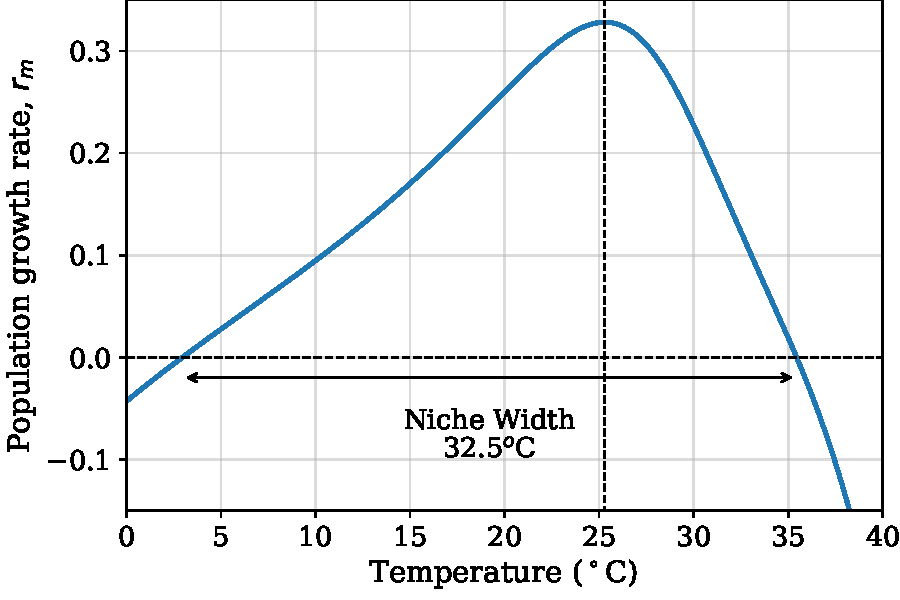
\includegraphics[width = .7\textwidth]{results/r_TPC.pdf}
	\caption{Illustration of the thermal niche of vector populations. We define the thermal niche of a vector population as the range of temperatures for which the vector population growth rate ($r_\text{m}$) is great than or equal to zero. Vector populations with a population growth rate less than zero will decline towards extinction}
\label{fig:ThermalNiche}
\end{figure} 

\subsection*{Sensitivity of the growth rate TPC to underlying traits}

In order to determine the traits driving the sensitivity of the TPC for population growth rate to thermal mismatches between between juvenile and adult traits, we assess the sensitivity of the model to temperature dependence of each parameter.

This can be determined by using the chain rule to determine the relative contribution of the temperature dependence of each parameter to the temperature dependence of population growth rate. The relative contribution of a parameter can be expressed as the product of the partial derivative of population growth rate  ($r_\text{m}$) with respect to a parameter and the derivative of that parameter with respect to temperature:

\begin{equation}\label{eq:sensitivity}
	\frac{\mathrm{d}r_\mathrm{m}}{\mathrm{d}T} = 
	\frac{\partial r_\mathrm{m}}{\partial b_{pk}} \frac{\mathrm{d}b_{pk}}{\mathrm{d}T} + 
	\frac{\partial r_\mathrm{m}}{\partial \alpha}\frac{\mathrm{d}\alpha}{\mathrm{d}T} + 
	\frac{\partial r_\mathrm{m}}{\partial z} \frac{\mathrm{d}z}{\mathrm{d}T} +
	\frac{\partial r_\mathrm{m}}{\partial z_J} \frac{\mathrm{d}z_J}{\mathrm{d}T} + 
	\frac{\partial r_\mathrm{m}}{\partial \kappa} \frac{\mathrm{d}\kappa}{\mathrm{d}T} 
\end{equation}

Having evaluated these terms (SI section S5), we can plot the relative contribution of each parameter to the thermal performance curve for population growth rate. The sensitivity of population growth rate to the thermal sensitivity of each parameter can be assessed by the deviation of the line for the partial derivative with respect to each parameter from zero. Furthermore, terms in equation \eqref{eq:sensitivity} can be combined according to life stage the trait is associated with. In the case of our mosquito example, development rate and juvenile mortality are the juvenile traits while adult mortality, fecundity, and rate of loss of fecundity are the adult traits. These together  determine the relative contribution of the thermal sensitivity of each life stage to the thermal sensitivity of population growth rate. 
%%%%%%%%%%%%%
%% Move to Supplemental %%
%%%%%%%%%%%%%

\begin{table}[ht]
\caption{{\bf The metabolic traits underlying vector fitness and abundance}. The parameter $B_0$ is the trait value at a $10^{\circ}$C ($T_\text{ref} = 283.15$ K, or $10^\circ C$), and along with the parameters $T_\text{opt}$, $E$, and $E_\text{D}$ (eqn \eqref{eq:TPCModel}; Fig. \ref{fig:TPCModel}) determines the TPC of each trait. The parameters $E$, and $E_D$ were respectively set to be the same across all traits ($T_\text{opt} = 26^\circ$C, $E = 0.6$eV and $E_\text{D} = 4$ eV), with $T_\text{opt}$ varied according to life stage to simulate mismatches. That the value of $\kappa$'s $B_0$ is a range reflects uncertainty about the temperature-dependence of this trait, which has been poorly studied empirically (Supplementary Information 2).}
\label{tab:traits}
\centering
\begin{tabular}{c p{4cm} p{8cm} l l l l } \toprule
% \multicolumn{7}{*}{TPC Parameters} \\
{\bf Parameter} & {\bf Units} & {\bf Description} & $B_0$ \\ \midrule
 $\alpha$ & days & Egg to adult development time & 10.0 \\
$b_\text{opt}$ & eggs $\times$ female $\times$ day$^{-1}$ & Peak 
reproductive rate & 10.0 \\
$z$ & days$^{-1}$ & Adult mortality rate & 0.03\\
$z_J$ & days$^{-1}$ & Mortality rate averaged across juvenile stages & 
0.05 \\
$\kappa$ & days$^{-1}$ & Fecundity loss rate & 0 -- 1 \\ \bottomrule
\end{tabular}

\end{table}
%%%%%%%%%%%%%
%% RESULTS %%
%%%%%%%%%%%%%

\section*{Results}

Both the thermal optimum and peak population growth are sensitive to mismatches (Fig. \ref{fig:ThermMM}). The thermal optimum ($T_\text{opt}$) (Fig. \ref{fig:ThermMM}B) increases asymptotically as the common thermal optimum of juvenile traits increases relative to that of adults. When the mismatch is such that juvenile traits peak at lower temperatures than adult traits, increasing the magnitude of mismatch decreases predicted ($T_\text{opt}$). When juvenile traits peak at higher temperatures than adult traits the relationship flips and the greater the mismatch the higher the predicted ($T_\text{opt}$). For the range of mismatches we explore ($-10^\circ$C to $+10^\circ$C) , $T_\text{opt}$ varies by about 12 $^\circ$C. The asymptotic nature of this change is expected to be a general feature across species because even if the thermal optimum of juvenile traits increases, each adult trait inherently declines rapidly with temperature beyond the adult thermal optimum (Fig. \ref{fig:TPCModel}; Fig. Sxx). Similarly, peak population growth ($r_\text{opt}$) also changes as the thermal optimum increases with physiological mismatch (Fig. \ref{fig:ThermMM}C). This is because of the ``hotter-is-better'' constraint built into the Sharpe-Schoolfield model \citep{Schoolfield1981} --- optimal rates inexorably rise with thermal optimum because of thermodynamic constraints, which has been shown to hold across a wide range of insect species \citep{Frazier2006}. 

The thermal niche width, the range of temperatures for which the intrinsic population growth rate is non-negative (Fig. \ref{fig:ThermalNiche}), also changes in response to physiological mismatches between juvenile and adult traits (Fig. \ref{fig:ThermMM}D). In this particular combination of species and its TPC parameterization, this variation spans about 20 $^\circ$C. This response of niche width to mismatch magnitude is also an asymptotic response for the same reason as the response of the $T_\text{opt}$ explained above. 

\begin{figure}[H] 
	\centering
	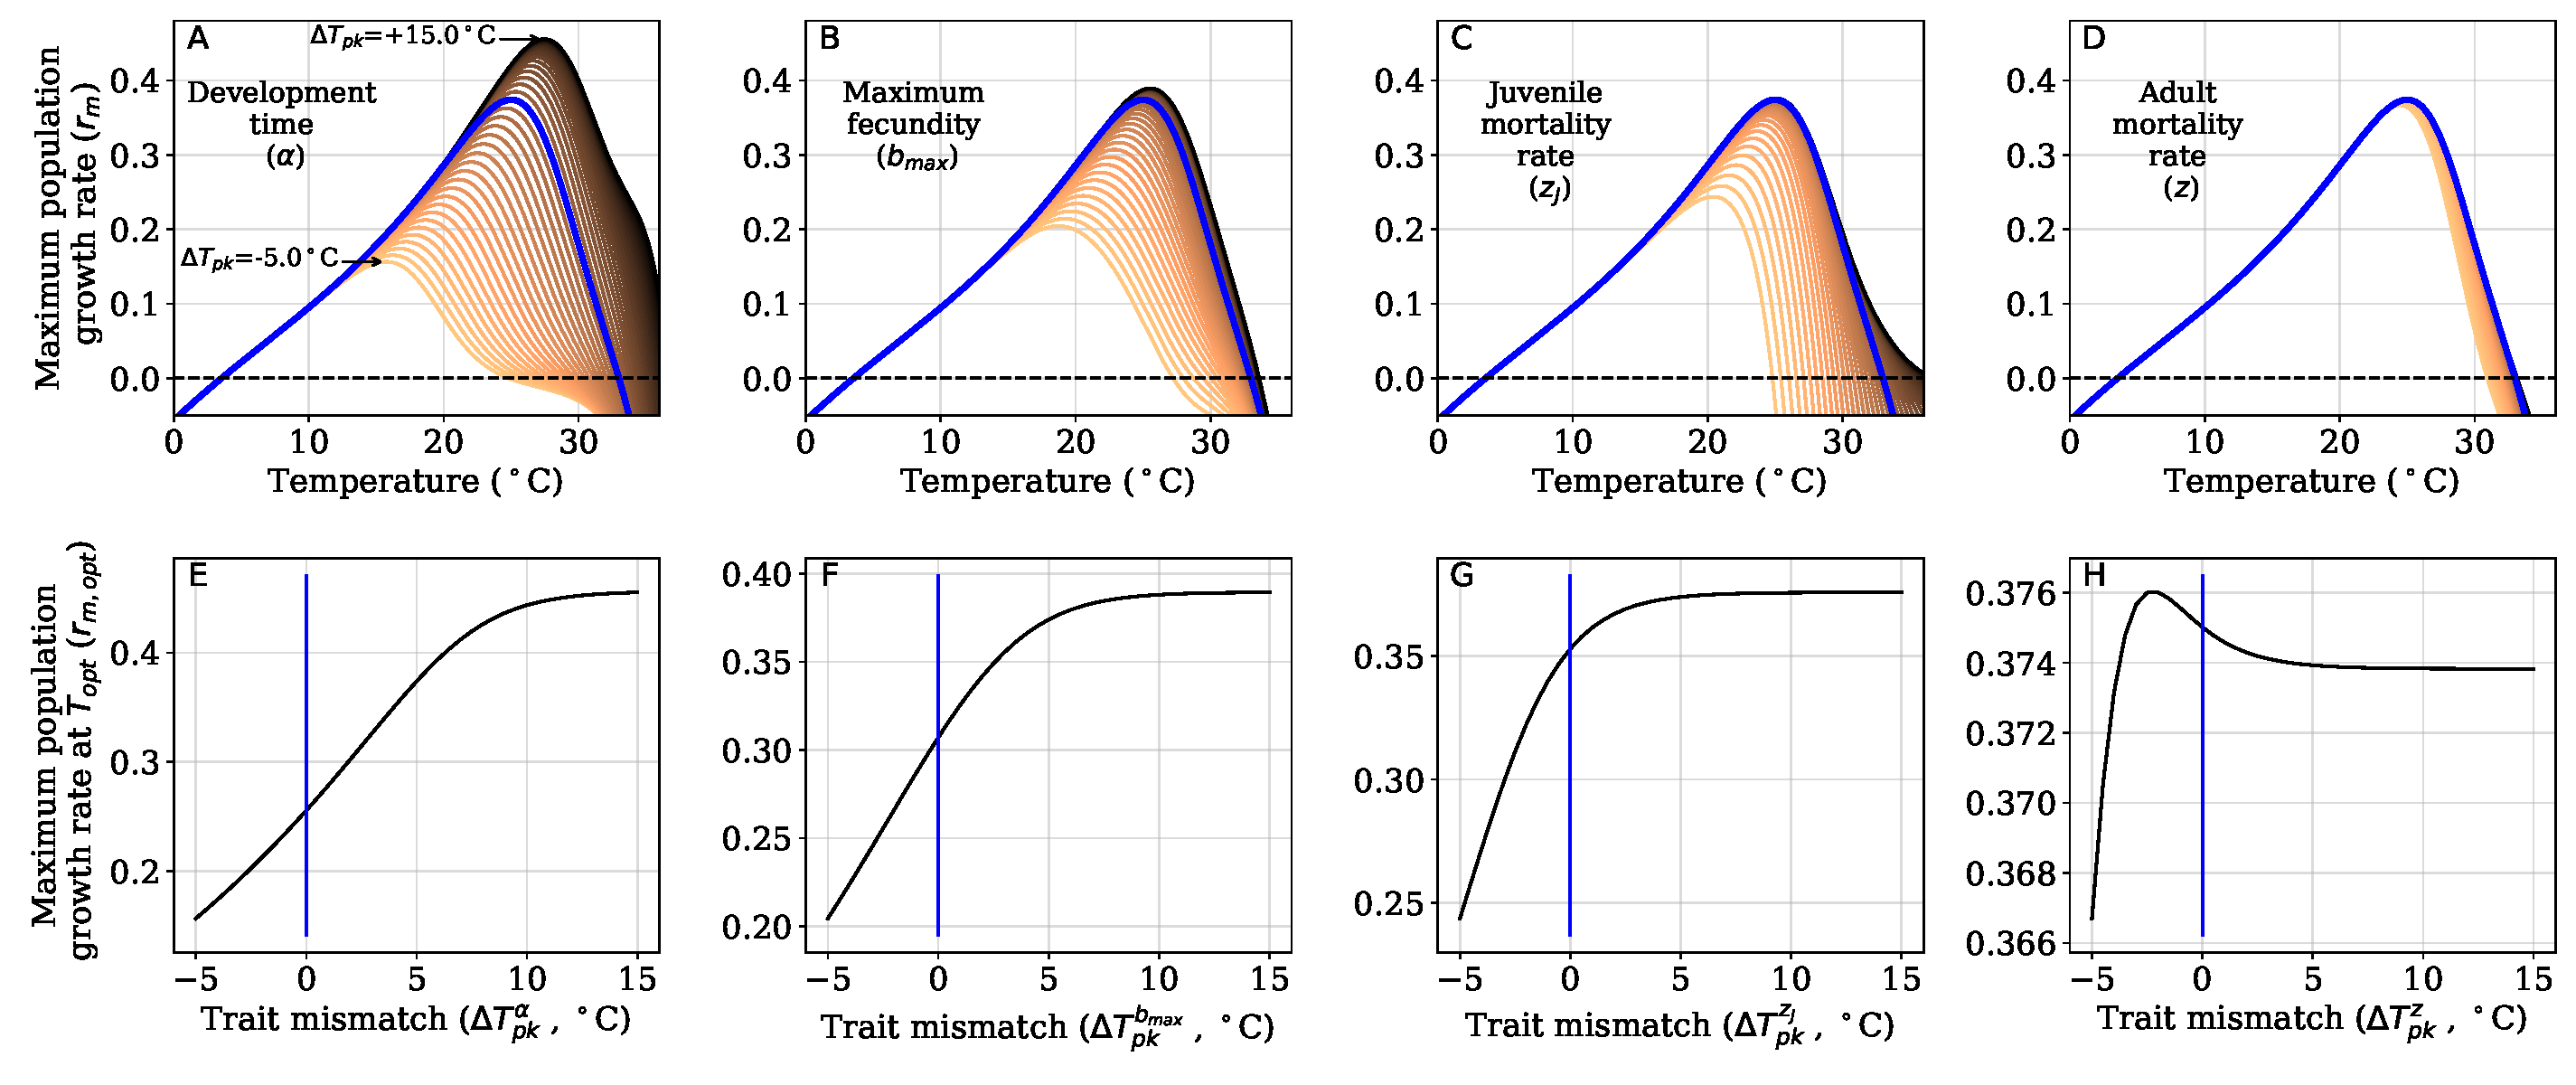
\includegraphics[width = .7\textwidth]{results/ThermMM.pdf}
	\caption{{\bf The impact of physiological mismatches in the thermal optima of juvenile and adult life stages on the population growth rate of arthropod vectors. A:} The temperature dependence of  population growth rate with differences in the thermal optima of juvenile traits from adult traits of $-10^\circ$C to $10^\circ$C. The thermal dependence of vector density with no mismatch between life stages is displayed as a solid black line. Blue lines represent how rm varies when adult trait optimum temperatures are higher than juvenile and red line represent mismatches in which the juvenile trait optimum temperatures are higher than the adult trait optimums. Underlying this patters are the relationships between mismatch and ($T_\text{opt}$) (B) and ($r_\text{opt}$) (C) {\bf B:} The impact of mismatches in the thermal optima of juvenile and adult traits on the thermal optima of the vector population growth rate ($T_\text{opt}$).  {\bf C:} The impact of mismatches in the thermal optima of juvenile and adult traits on the peak vector population growth rate ($r_\text{opt}$). {\bf D:} The relationship between the thermal optimum ($T_\text{opt}$) and range of temperatures for which population growth rate is greater than 0.
	\todonum[inline,caption={}]{To aid reference to the non mismatch scenario, add marker at no mismatch point in subplots B-D. Add scale to A}}
\label{fig:ThermMM}
\end{figure} 

The magnitude of sensitivity of the growth rate TPC (both in terms of optimum and niche width) to magnitude of physiological mismatch is expected to vary with the relative contributions of the different adult and juvenile traits. We find that relative to adult traits, the temperature dependence of juvenile traits contribute more to the TPC of growth rate (Fig. \ref{fig:r_sens}B) over a temperature range of 0--35$^\circ$C. This is largely driven by the contribution of juvenile development rate ($\alpha$), with juvenile mortality also having an increasing influence at extreme temperatures (Fig. \ref{fig:r_sens}A). This is also likely to be a fairly general result because arthropod population growth rates are typically expected depend strongly on juvenile development rate and mortality \citep{Birch1948}.

\begin{figure}[H] 
	\centering
	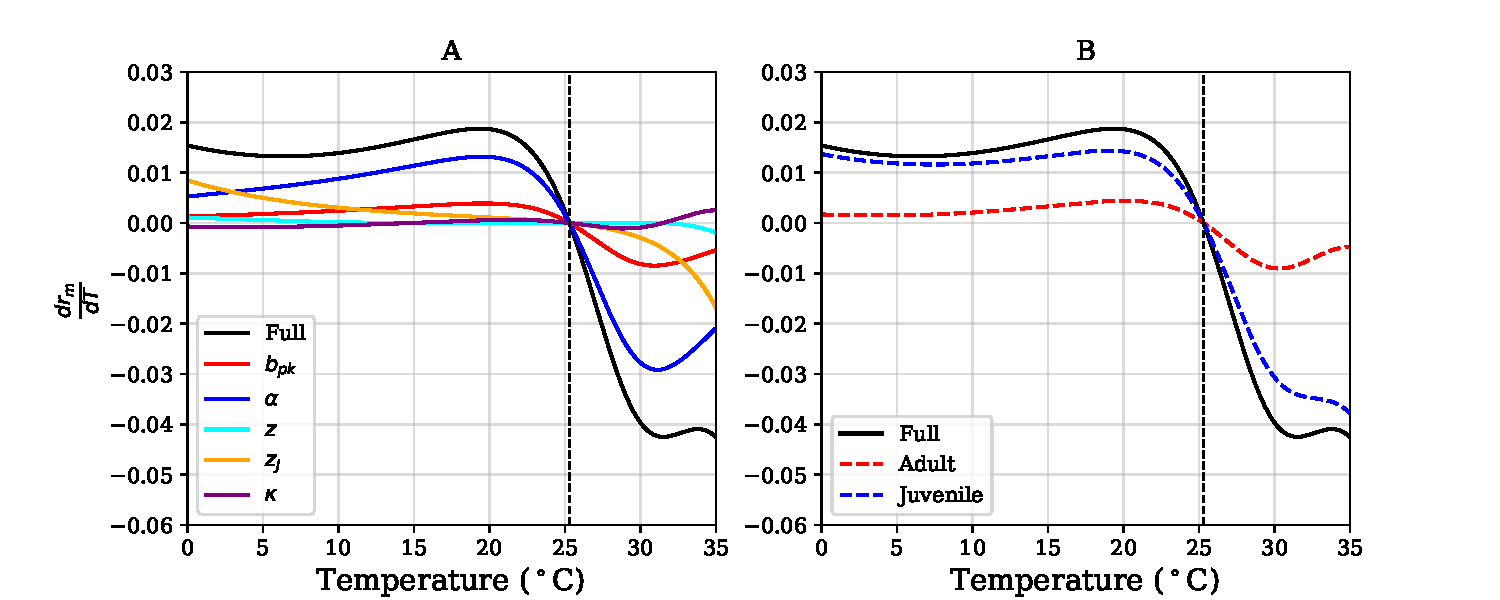
\includegraphics[width = .8\textwidth]{results/r_sens1.pdf}
	\caption{{\bf The temperature dependence of growth rate of insect vector populations and its sensitivity to underlying traits.} Greater deviation from zero indicates greater contribution of the traits to the temperature-dependence of population growth rate.
	{\bf A:} The contributions of the temperature-dependence of each life history trait to the temperature-dependence of population growth rate.
	{\bf B:} The summed contributions of the juvenile and adult life history traits to the temperature dependence of the population growth rate.}
\label{fig:r_sens}
\end{figure} 

%%%%%%%%%%%%%%%%
%% DISCUSSION %%
%%%%%%%%%%%%%%%%

\section*{Discussion}
% \cite{Mordecai2017,White2011a,Parham2012,Ferguson2010}
% \cite{Christiansen-Jucht2014a}

The population dynamics of disease vectors are essential to modelling the transmission dynamics of vector borne diseases in animals and plants. Our results highlight the importance of physiological mismatches --- differences in the thermal performance curves of different traits --- on these dynamics. More specifically, we have shown that, mismatches between juvenile and adult life history traits are likely to be a particularly important factor underlying the temperature dependence of vector population growth rate. 

The sensitivity of the thermal optimum and niche width of the TPC for vector population growth rate to the magnitude of physiological mismatches between different vector life stages highlights the potential importance of stage-specific differences in environmental niche to vector population dynamics. Assuming that the thermal optimum and niche width of traits of different life stages reflect (through life history adaptation and phenotypic plasticity or acclimation) the local environmental temperature range experienced by those stages, quantifying the effects of mismatches in this way provides a new and important tool for understanding the effects of climate change on population dynamics of disease vectors. Such differences in the temperatures experienced by different life stages are expected to be common in arthropods. 

Furthermore, our modelling framework provides a relatively simple approach for incorporating a mechanistic model of thermal dependence of abundance intro disease transmission models. By not requiring complex simulations of stage-structured vector population dynamics, this model may facilitate the projection of vector population dynamics, and by extension, epidemiological measures such as $R_0$, across geographical and environmental space. The incorporation of physiological mismatches in this framework may also contribute to our undestanding of vector population dyanmics and the responses of vector populations, and by extension vector-borne disease dyanmics, to a changing climate.

Our model indicates that across a broad range of temperatures, juvenile traits are more important than adult traits in determining the population growth rate of vectors, and that both the thermal optimum and peak vector population growth rate are sensitive to thermal mismatches between juvenile and adult life stages. In the case of this particular vector (mosquito) and parameterizations used here to illustrate the framework, we find that  this is largely driven by the contribution of juvenile development rate ($\alpha$), with juvenile mortality also having an increasing influence at extreme temperatures (Fig. \ref{fig:r_sens}A). This is likely to be a fairly general result because arthropod population growth rates typically depend strongly on juvenile development rate and mortality \hlfix{[Refs]}.

\hlfix{Our framework requires data on the thermal responses of a small set of key, commonly-measured life history parameters, and in principle, should be applicable to any vector population with stage-structured life history. However, to confidently fit appropriate TPCs, we would need robust data covering an appropriate range of temperatures, which is difficult to achieve. Furthermore, for many species of disease vector the data for the full complement of traits has not been published.}

A notable absence for all species of vector is data on the rate of loss of fecundity ($\kappa$), and especially how this trait responds to temperature. A experimental study by \citet{Stavrinides2011} showed that the fecundity schedule for three species of mite are sensitive to temperature.

\hlfix{The results of this study indicate that the differences in the environmental conditions experienced by juvenile and adult lifestages of vectors warrent greater consideration. This is especially true when considering the impact of temperature on vector populations, such as in the context of climate change and the shifting geographic distributions of vectors and the pathogens they transmit.}{Highlighted passages are work in progress}

\begin{itemize}
\item Talk about trait data and $\kappa$
\item Discuss the need for robust data on traits across appropriate ranges of temperatures to quantify mismatches --- also need for data in a wide range of species 
\item Maybe talk about modelling explicitly juv vs adult environmental differences --- not just differences in TPCs.    
\item \hlfix{Talk about non-sharpe-schoolfield TPC models, and whether hotter is better is likely to be biologically relevant.}{For SP}
\end{itemize}

\bibliographystyle{ecology} 
\bibliography{VecMismatch}

\pagebreak

% \section*{Figures}
 
\end{document}
